\chapter{things hidden}
\label{sec:things_hidden}
\lhead[tempest]{}
\lstset{style=6502Style}


These appear to be enemy attack ships of a previously unknown configuration defined in the source
file \icode{ALVROM.MAC}. An assembly flag excluded these objects from the final release of the game
but their full specification is available to us in a series of vector commands. This has enabled the
us to painstakingly reconstruct the artefacts using modern equipment. We present them here to the reading public for the first time.

\begin{figure}[H]
  \centering
        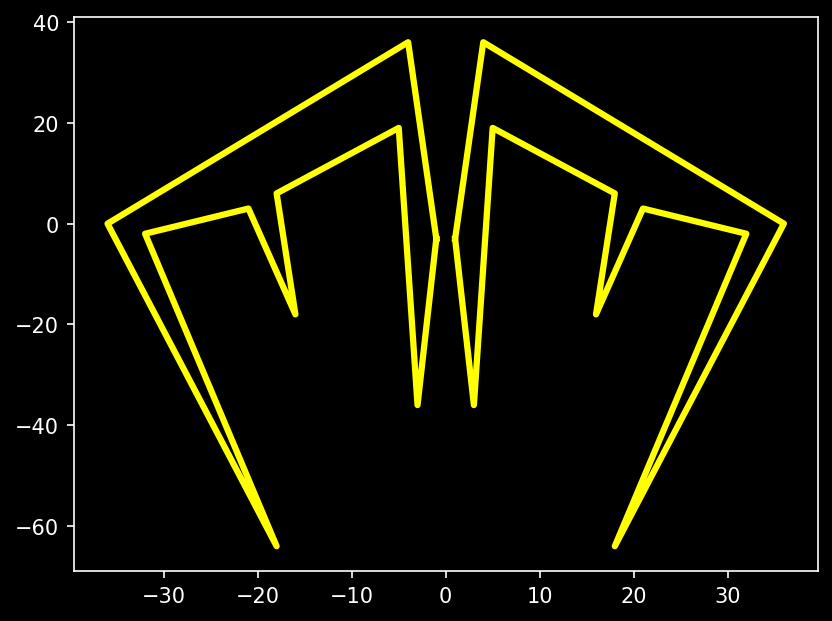
\includegraphics[width=4.22cm]{src/tempest_unused/ENER21.png}%
        \hspace{0.2cm}
        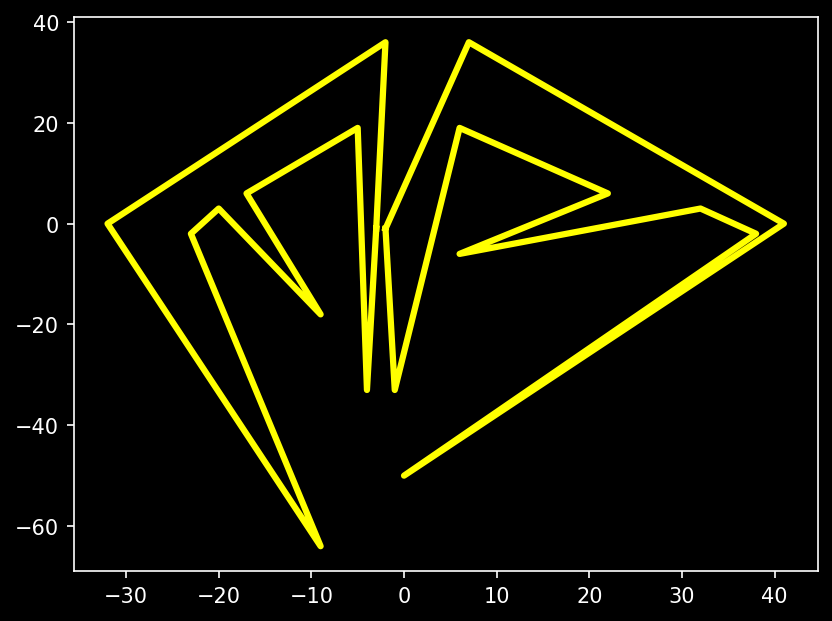
\includegraphics[width=4.22cm]{src/tempest_unused/ENER22.png}%
        \hspace{0.2cm}
        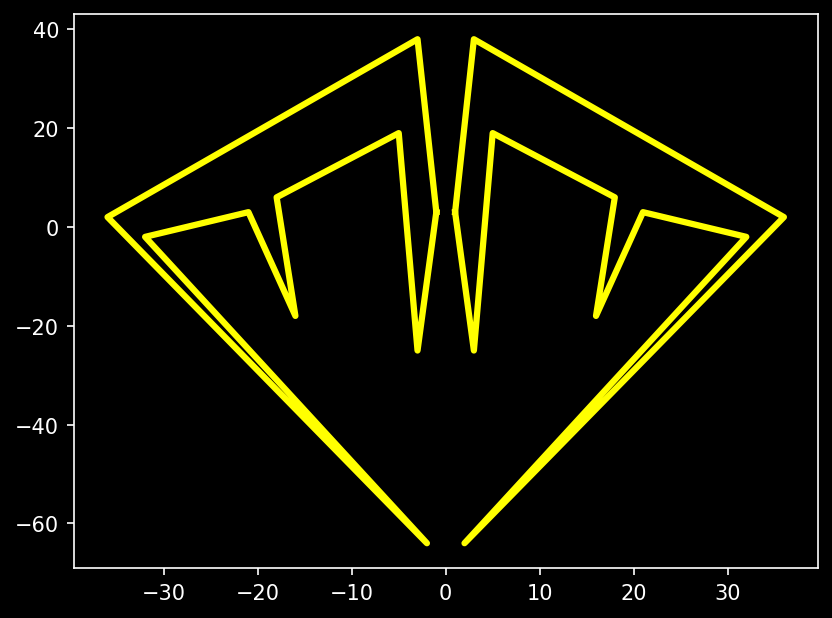
\includegraphics[width=4.22cm]{src/tempest_unused/ENER23.png}%
        \hspace{0.2cm}
        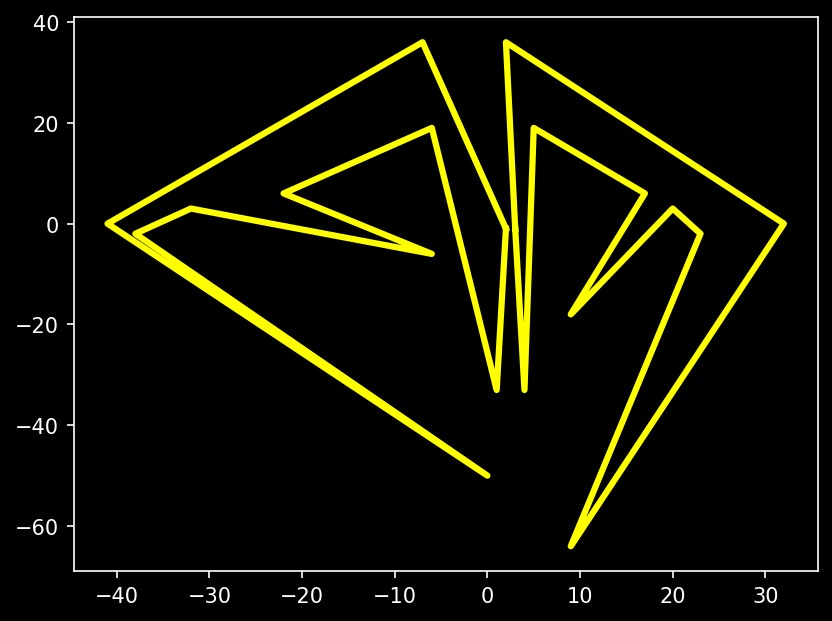
\includegraphics[width=4.22cm]{src/tempest_unused/ENER24.png}%
  \caption*{ENER21 to ENER24 in ALVROM.MAC.}
\end{figure}

\vspace{-0.5cm}
The best of our finds is a clear predecessor to the iconic 'claw' ship. Each is defined
using an array of X/Y co-ordinates that a macro by the name of \icode{CALVEC} encodes into a list
of vector commands. For example, the first image in Figure 2 above is given as follows in
\href{https://github.com/historicalsource/tempest/blob/6c783bee488ed736fc3fdc3a81fdc412c3bec386/ALVROM.MAC#L1483}{\textcolor{blue}{lines 1483-1512} in \icode{ALVROM.MAC}}:
\footnote{https://github.com/historicalsource/tempest/blob/
6c783bee488ed736fc3fdc3a81fdc412c3bec386/
ALVROM.MAC\#L1483}
\begin{lstlisting}
ENER21:
  ICALVE               ; X:0   Y:0     
  CALVEC -1,-3         ; X:-1  Y:-3     
  .BRITE=VARBRT        ; Set brightness to 1
  CALVEC -4,24.        ; X:-4  Y:36
  CALVEC -24.,0        ; X:-36 Y:0
  CALVEC -12.,-40.     ; X:-18 Y:-64
  CALVEC -20.,-2       ; X:-32 Y:-2
  CALVEC -15.,3        ; X:-21 Y:3
  CALVEC -10.,-12.     ; X:-16 Y:-18
  CALVEC -12.,6        ; X:-18 Y:6
  CALVEC -5,13.        ; X:-5  Y:19
  CALVEC -3,-24.       ; X:-3  Y:-36
  CALVEC -1,-3         ; X:-1  Y:-3
  .BRITE=0             ; Set brightness to 0 
  CALVEC 1,-3          ; X:1   Y:-3
  .BRITE=VARBRT        ; Set brightness to 1 
  CALVEC 3,-24.        ; X:3   Y:-36
  CALVEC 5,13.         ; X:5   Y:19
  CALVEC 12.,6         ; X:18  Y:6
  CALVEC 10.,-12.      ; X:16  Y:-18
  CALVEC 15.,3         ; X:21  Y:3
  CALVEC 20.,-2        ; X:32  Y:-2
  CALVEC 12.,-40.      ; X:18  Y:-64
  CALVEC 24.,0         ; X:36  Y:0
  CALVEC 4,24.         ; X:4   Y:36
  CALVEC 1,-3          ; X:1   Y:-3
  .BRITE=0             ; Set brightness to 0 
  CALVEC NXE,0         ; X: 0   Y:0     
  RTSL
\end{lstlisting}

\vspace{0.3cm}
The listing gives X and Y co-ordinates in hex, which we can readily plot as vertices on a graph. During
assembly these values were converted to \href{https://arcarc.xmission.com/Tech/neilw_xy.txt}{\textcolor{blue}{'relative draw'}}\footnote{https://arcarc.xmission.com/Tech/neilw\_xy.txt} vector commands for use by the Atari Analogue Vector Generator (AVG).
These encode \icode{X} and \icode{Y} vectors, along with an intensity value \icode{I} as follows:
\vspace{-0.2cm}
\begin{figure}[H]
  {
    \setlength{\tabcolsep}{3.0pt}
    \setlength\cmidrulewidth{\heavyrulewidth} % Make cmidrule = 
    \begin{adjustbox}{width=8.5cm,center}
      \begin{tabular}{llll}
        \toprule
          &   &   & Vector Command Bits\\
        X & Y & I & \icode{000Y YYYY YYYY YYYY IIIX XXXX XXXX XXXX} \\
        \midrule
        \icode{FF} &\icode{FD} & \icode{00} & \icode{0001 1111 1111 1100 0001 1111 1111 1111} \\
        \addlinespace
        \bottomrule
      \end{tabular}
    \end{adjustbox}
  }
\end{figure}
\vspace{-0.54cm}

The values chosen above are not arbitrary: \icode{X} is -1 (\icode{FF}) and \icode{Y} is -3 (\icode{FD}). Together with an
assumed intensity value of \icode{0} these form the first entry in \icode{ENER21}: \icode{CALVEC -1,-3},
which gets encoded in \href{https://en.wikipedia.org/wiki/Ones%27_complement}{\textcolor{blue}{one's complement}}
\footnote{https://en.wikipedia.org/wiki/Ones\%27\_complement}
for the thirteen bits of each value: \icode{1FFD 1FFF}. 

There are twelve other finds of interest given below. Unlike the set in Figure 2 above, none of these resemble early
iterations of the player's 'claw'. All our finds appear in an area of the source code described as \icode{ENEMY PICTURES}
and are more likely to be just that: a set of alien enemies for a very early iteration of Tempest that according to
programmer David Theurer was a 
\href{https://arcadeblogger.com/2018/01/19/atari-tempest-dave-theurers-masterpiece/}{\textcolor{blue}{‘First Person Space Invaders’}}.
\footnote{https://arcadeblogger.com/2018/01/19/atari-tempest-dave-theurers-masterpiece/}
\vspace{-0.3cm}
\begin{figure}[H]
  {
        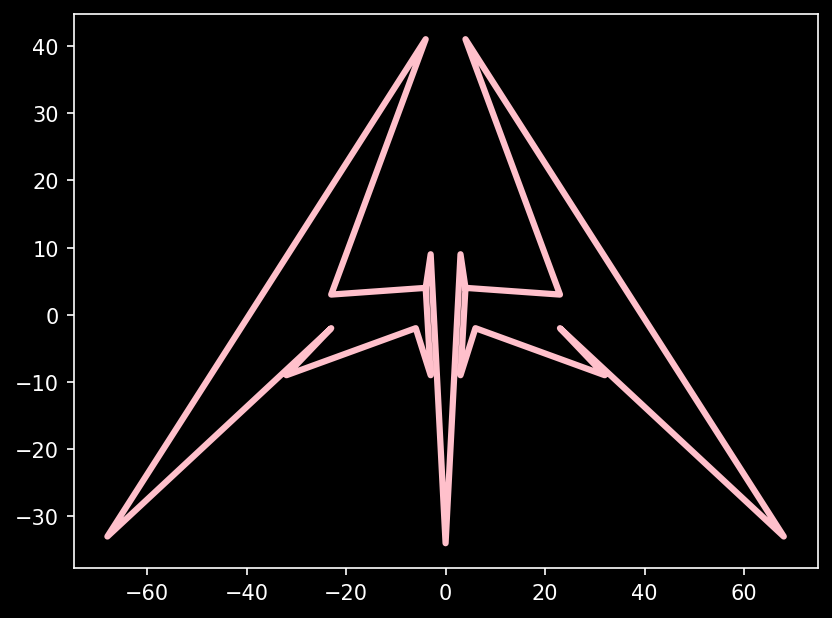
\includegraphics[width=3.22cm]{src/tempest_unused/ENER11.png}%
        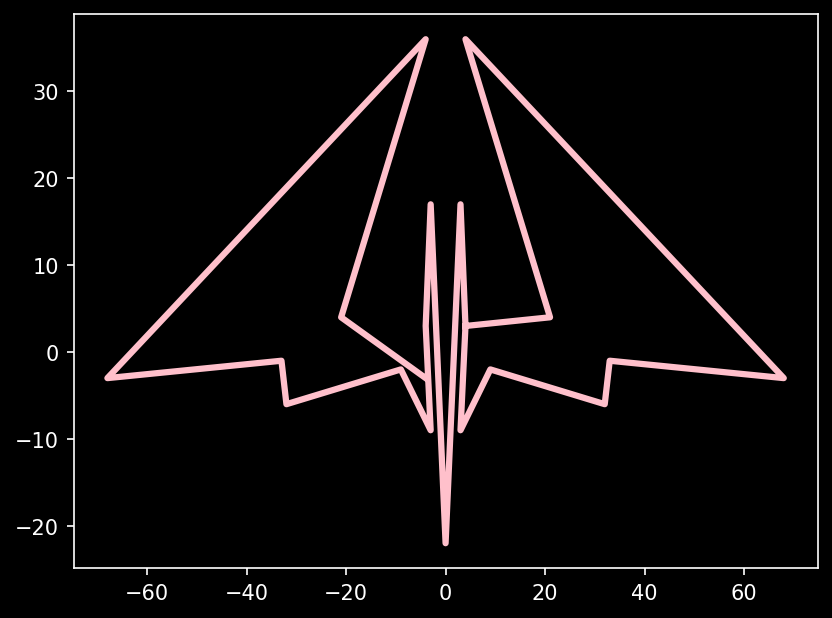
\includegraphics[width=3.22cm]{src/tempest_unused/ENER12.png}%
        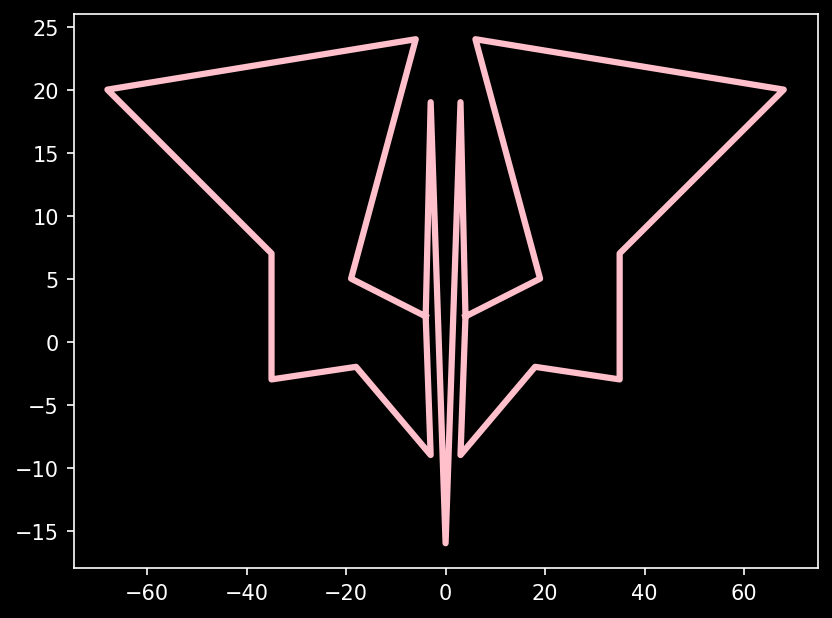
\includegraphics[width=3.22cm]{src/tempest_unused/ENER13.png}%
        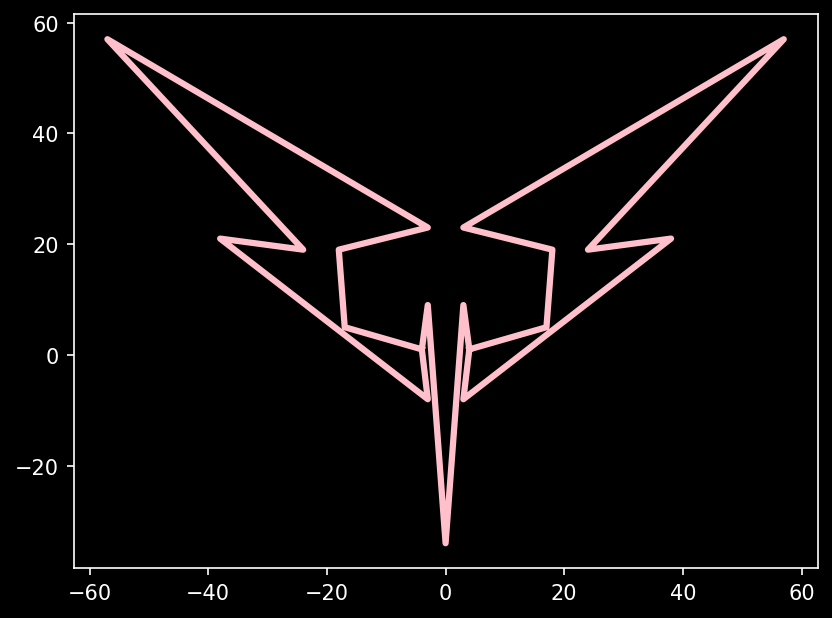
\includegraphics[width=3.22cm]{src/tempest_unused/ENER14.png}%
        \vspace{-0.2cm}
  }\caption*{ENER11 to ENER14 in ALVROM.MAC.}
\end{figure}
\begin{figure}[H]
  {
        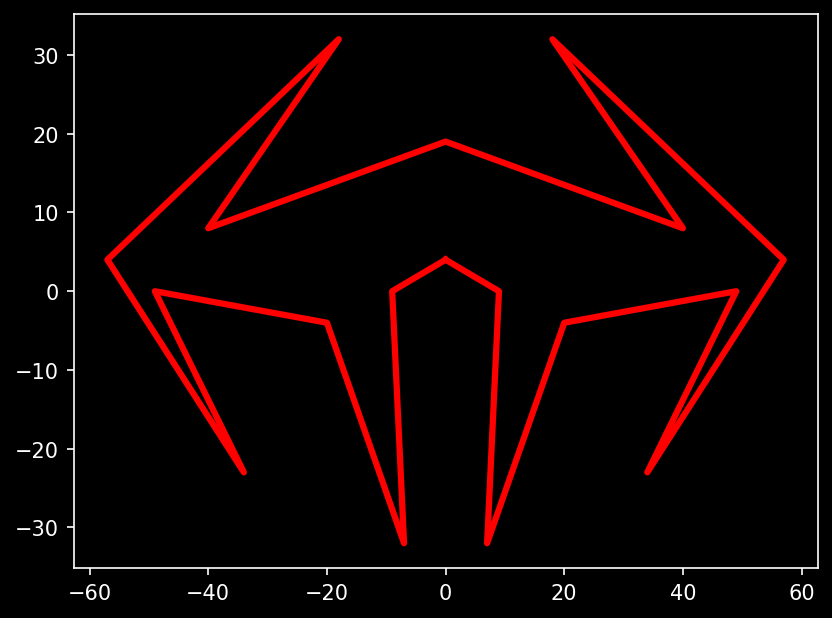
\includegraphics[width=3.22cm]{src/tempest_unused/ENER41.png}%
        \hspace{-0.2cm}
        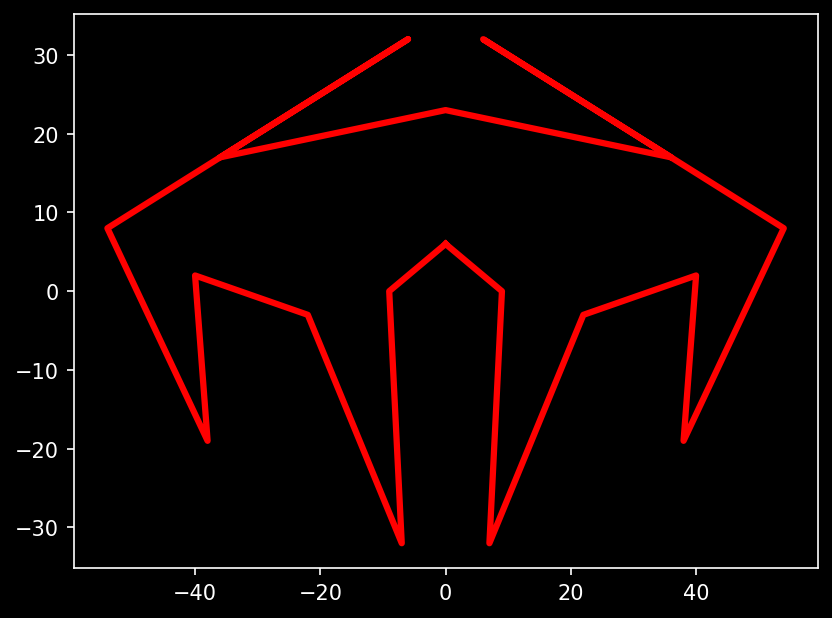
\includegraphics[width=3.22cm]{src/tempest_unused/ENER42.png}%
        \hspace{-0.2cm}
        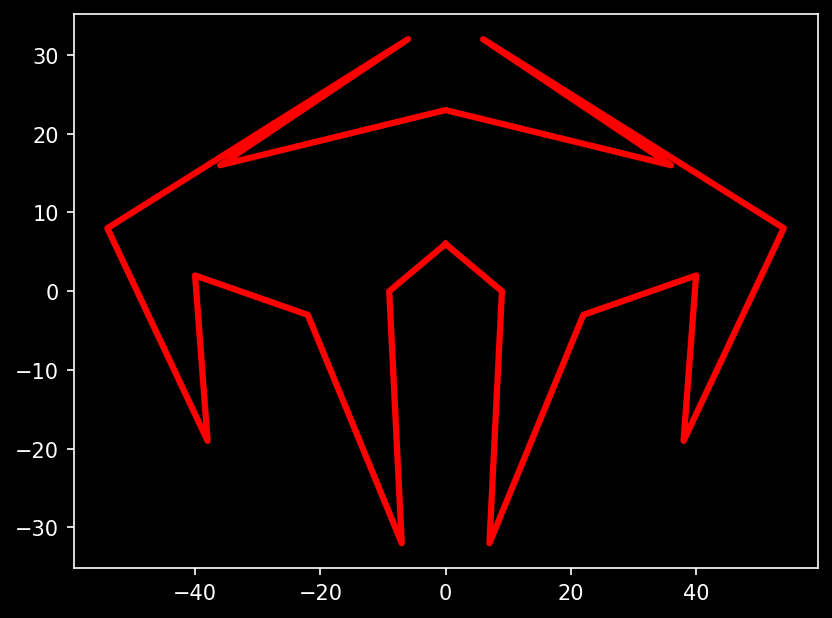
\includegraphics[width=3.22cm]{src/tempest_unused/ENER43.png}%
        \hspace{-0.2cm}
        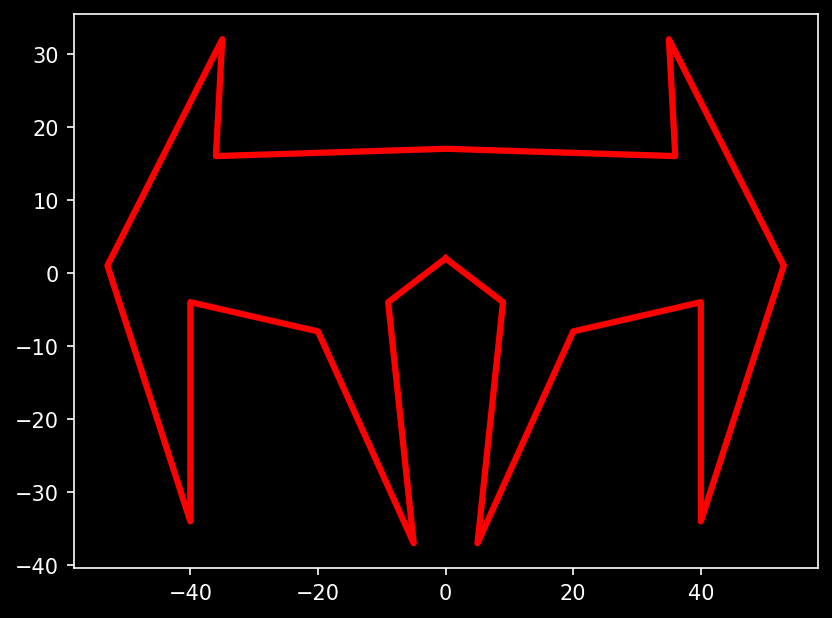
\includegraphics[width=3.22cm]{src/tempest_unused/ENER44.png}%
        \vspace{-0.2cm}
  }\caption*{ENER41 to ENER44 in ALVROM.MAC.}
\end{figure}
\begin{figure}[H]
  {
        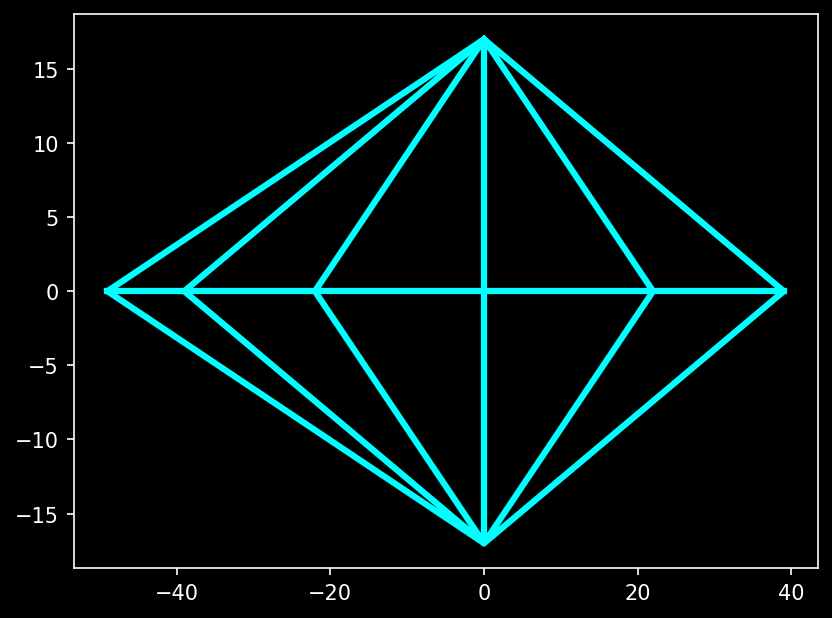
\includegraphics[width=3.22cm]{src/tempest_unused/SAU.png}%
        \hspace{-0.2cm}
        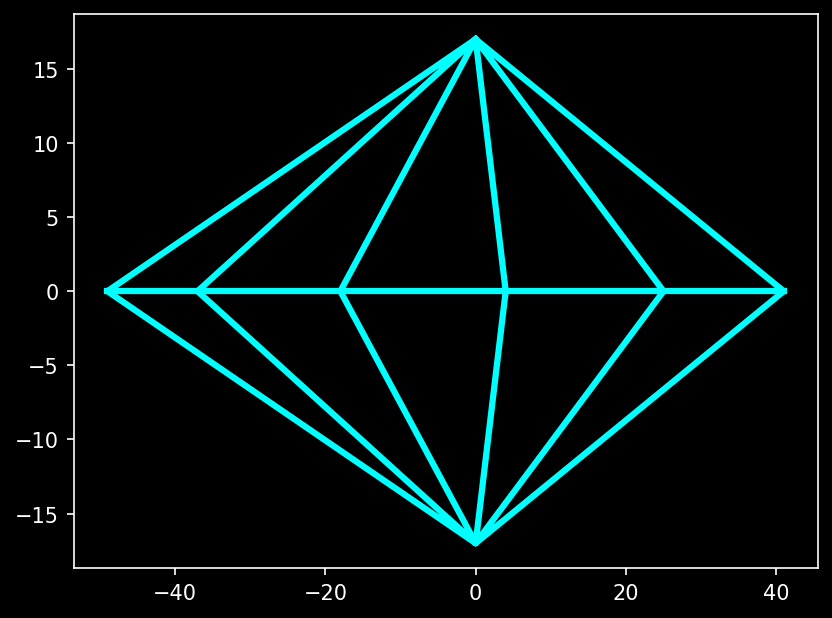
\includegraphics[width=3.22cm]{src/tempest_unused/SA2.png}%
        \hspace{-0.2cm}
        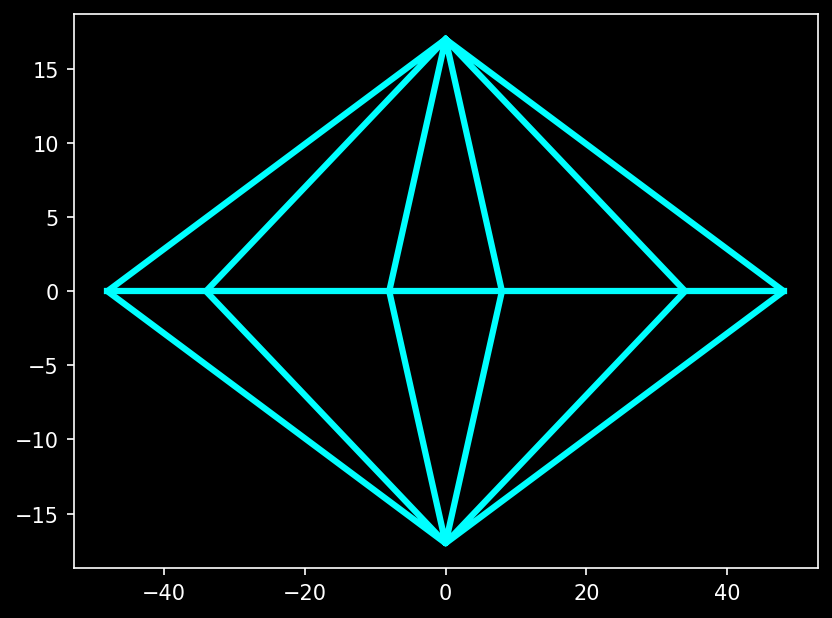
\includegraphics[width=3.22cm]{src/tempest_unused/SA3.png}%
        \hspace{-0.2cm}
        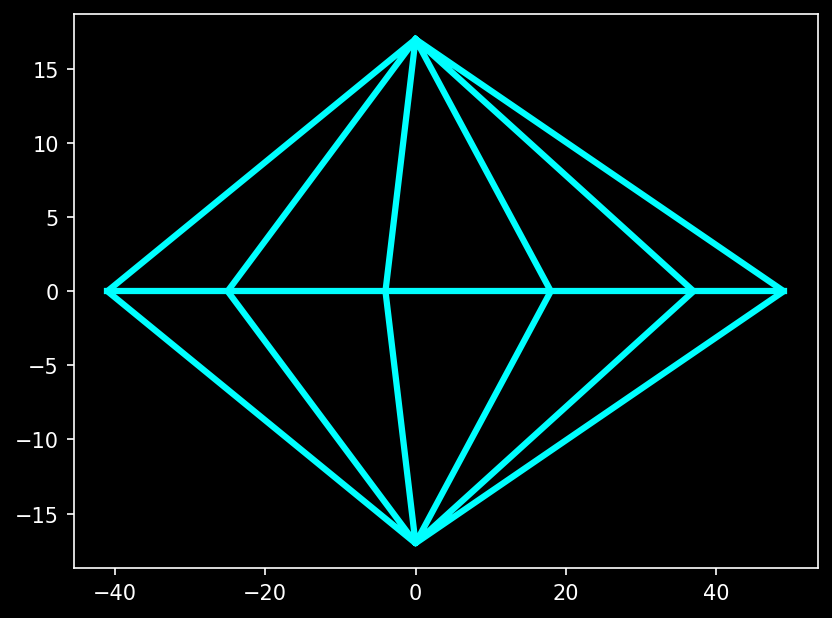
\includegraphics[width=3.22cm]{src/tempest_unused/SA4.png}%
        \vspace{-0.2cm}
  }\caption*{SAU to SA4 in ALVROM.MAC.}
\end{figure}

